\section{Nuclear Fuel Cycle}

\subsection{The Nuclear Fuel Cycle}

\begin{definition}
    The nuclear fuel cycle, also called nuclear fuel chain, is the progression of nuclear fuel through a series of differing stages. 
\end{definition}

\begin{itemize}
    \item FRONT END: the preparation of the fuel
    \item BACK END: safely manage, contain, and either reprocess or dispose of spent nuclear fuel
\end{itemize}

\begin{itemize}
    \item not reprocessed: {\itshape Open Fuel Cycle}
    \item reprocessed: {\itshape Closed Fuel Cycle}
\end{itemize}

\begin{figure}[H]
    \centering
    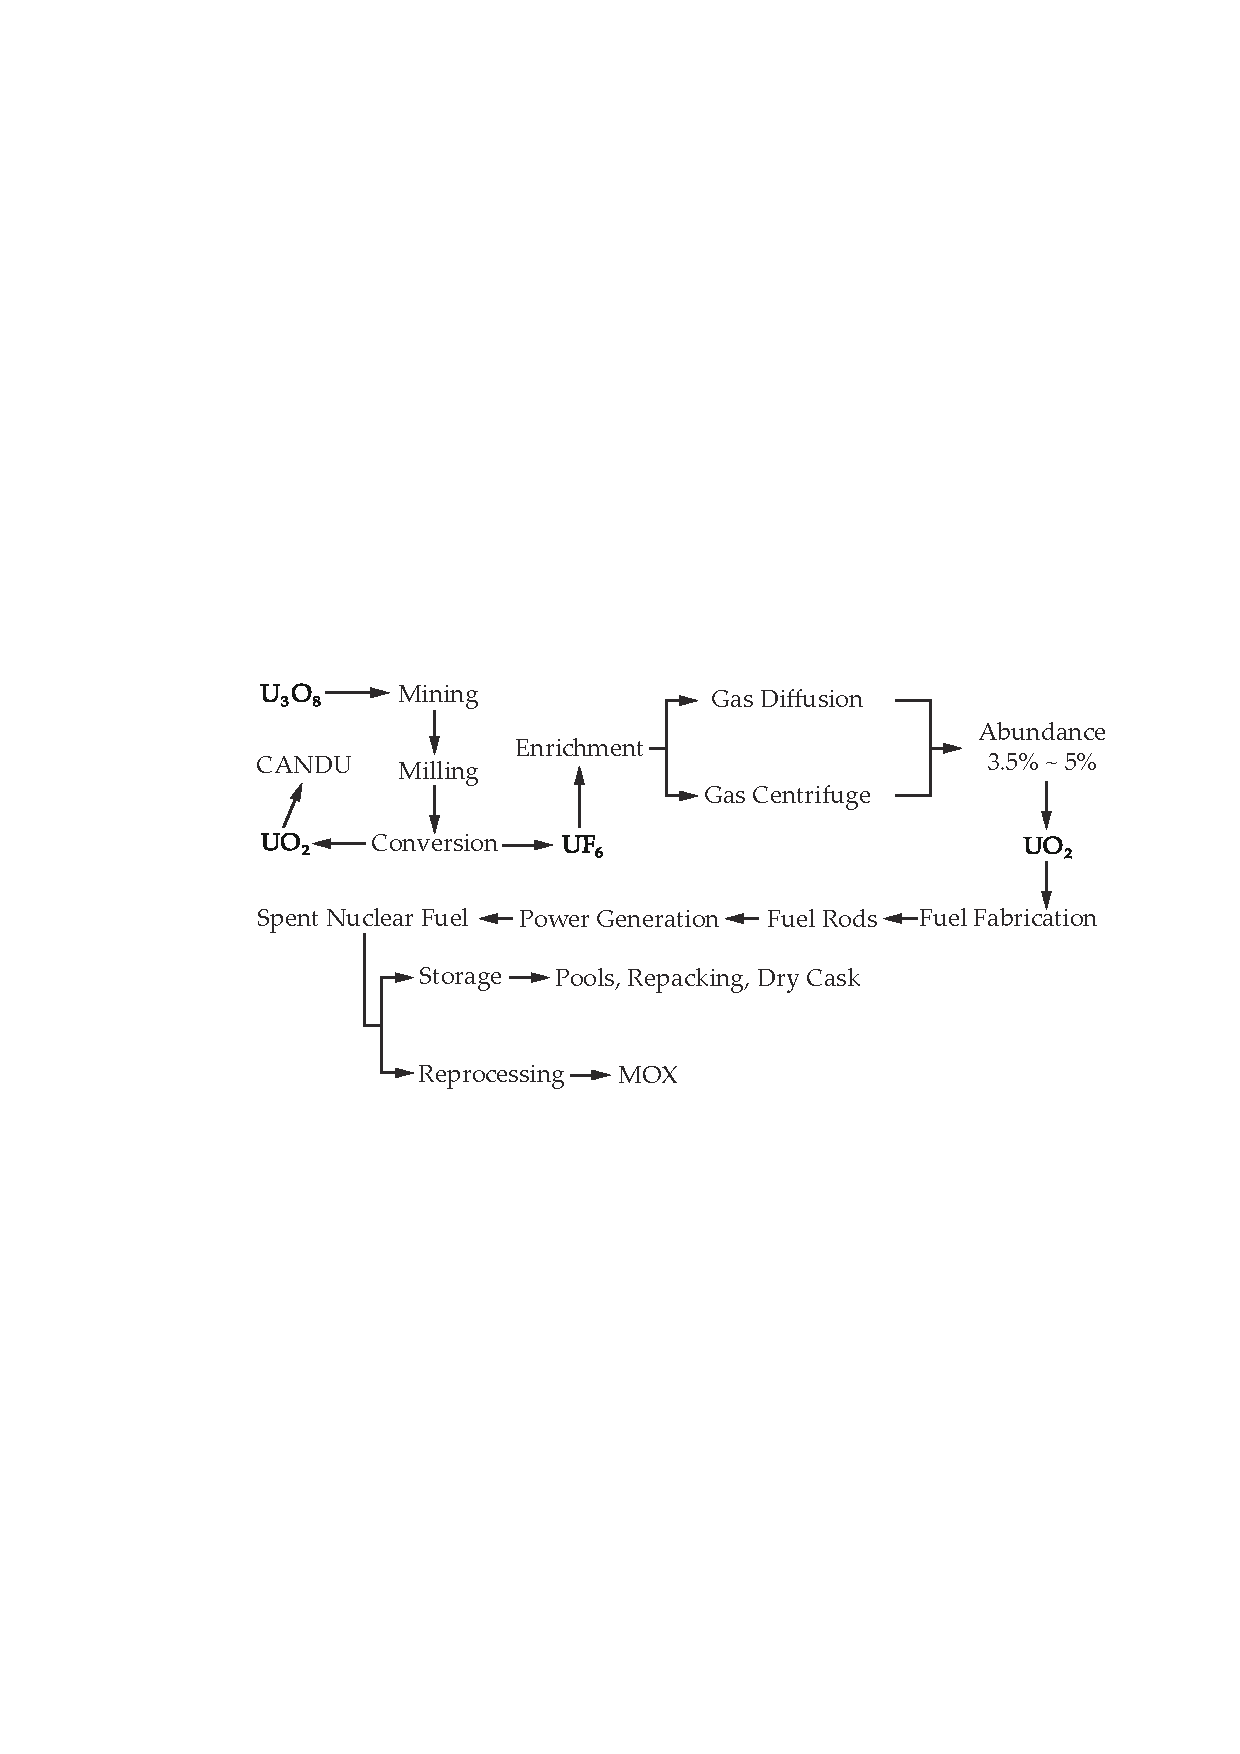
\includegraphics[scale=0.8]{figures/nuclear_fuel_cycle.pdf}
    \caption{The Nuclear Fuel Cycle}
\end{figure}

\subsection{Isotope Separation}

\begin{definition}
    Isotope separation is the process of concentrating specific isotopes of a chemical element by removing other isotopes.
\end{definition}

Isotope separation method:
\begin{itemize}
    \item Gas diffusion
    \item Gas centrifuge
    \item Aerodynamic processes
    \item Laser techniques
    \item Chemical methods
    \item Plasma separation process
    \item Thermal diffusion method
\end{itemize}

\subsubsection*{Gas diffusion}

When mixed gas reached the thermodynamic balance. The ${}^{235}{\rm UF_6}$ and ${}^{238}{\rm UF_6}$ have the same average kinetic energy but different velocity ({\bfseries Semi-Permeable Membranes, Micropores}). 

Conditions:
\begin{enumerate}
    \item Low pressure
    \item Keep aperture small
\end{enumerate}

The process is easy but economics is low.

\subsubsection*{Gas centrifuge}

The gas centrifuge process uses a large number of rotating cylinders in series and parallel formations.

High efficiency, Very economic, but highly depend on the strength of material.

\subsubsection*{Others}

\begin{itemize}
    \item Aerodynamic processes: Gas mixture expand through the slit nozzle, different centrifugal forces to partially separate isotopes
    \item Laser techniques: Selective excitation of isotopic atoms or isotopic containing compound molecules by a laser beam (Low cost but low efficiency)
    \item Chemical methods: The isotopic distribution in each reaction molecule is not equal probability during the isotopic chemical exchange reaction
    \item Plasma separation process: Plasma rotation and ion cyclotron resonance in the electromagnetic field
    \item Thermal diffusion method: When there is a temperature gradient in a homogeneous mixture of gases or liquids, the light components will be concentrated in hot regions and the heavy components will be concentrated in cold regions
\end{itemize}

\subsection{Nuclear Fuel Reprocessing}

Fuel Reprocessing \& Radioactive Waste Disposal

\begin{itemize}
    \item \faGrinBeam[regular]: Recover fissile material for energy extraction
    \item \faGrinBeamSweat[regular]: Economic disadvantage and political risks
\end{itemize}

\subsubsection*{Fuel Reprocessing}

\begin{itemize}
    \item Solvent extraction
    \item Plutonium and Uranium Recovery by Extraction, {\itshape PUREX}
\end{itemize}

\subsubsection*{Radioactive Waste Disposal}

\begin{itemize}
    \item High-level waste
    \begin{itemize}
        \item Without reprocessing: place in suitable containers and bury in some stable geological settings
        \item Be reprocessed: liquid form can be made into glass or surround beads of waste with layers of ceramic, then place in suitable containers and bury
    \end{itemize}
    \item Transuranic (TRU) waste
    \item Low-level waste
    \begin{itemize}
        \item Place in drums and shipped off-site to waste depositories
    \end{itemize}
    \item Mine and mill tailings
\end{itemize}
